
%(BEGIN_QUESTION)
% Copyright 2013, Tony R. Kuphaldt, released under the Creative Commons Attribution License (v 1.0)
% This means you may do almost anything with this work of mine, so long as you give me proper credit

One day the trend on a retort temperature monitoring system is seen to exhibit a ``noisy'' signal, which operations personnel have never noticed before.  According to them, this trend recorder's trace is always smooth, never noisy:

$$\includegraphics[width=15.5cm]{i03574x01.eps}$$

The loop sheet for this monitoring system is shown here:

$$\includegraphics[width=15.5cm]{i0011rx01.eps}$$

\filbreak

Explain how you would proceed to troubleshoot this problem, specifying what equipment you might use to do so.

\underbar{file i03574}
%(END_QUESTION)





%(BEGIN_ANSWER)

Temperature processes are naturally slow to change, and so the presence of high-frequency noise is simply not possible in the actual process variable (temperature).  Therefore, we know the noise must represent an equipment problem of some sort, causing a noisy PV {\it signal}.
 
\vskip 10pt

Since a noisy electronic signal is really nothing more than {\it AC} superimposed on the DC signal, we may use any test equipment capable of measuring AC to track the location of the problem.  Some modern digital multimeters are really good at discriminiating between AC and DC in voltage and current measurements, meaning we can set one of these meters to measure AC and it will {\it only} register the noise within the signal, rejecting the DC component of the signal.

\vskip 10pt

Therefore, a good test would be to use a DMM set to measure AC millivolts, and measure voltage signals at these points of the circuit:

\begin{itemize}
\item{} At the input terminals of TT-14 (to see if the thermocouple is picking up AC noise)
\item{} Between either input terminal of TT-14 and earth ground (to see if the thermocouple if picking up common-mode AC noise)
\item{} Between the (+) and (Gnd) terminals on the paperless chart recorder, to see if a noisy signal is present at the input of the recorder
\item{} Across the terminals of the loop power supply, to see if it is noisy itself
\end{itemize}

%(END_ANSWER)





%(BEGIN_NOTES)



%(END_NOTES)


